\section{Motivation}

\begin{frame}
\frametitle{Roles in Development Process}
\begin{center}
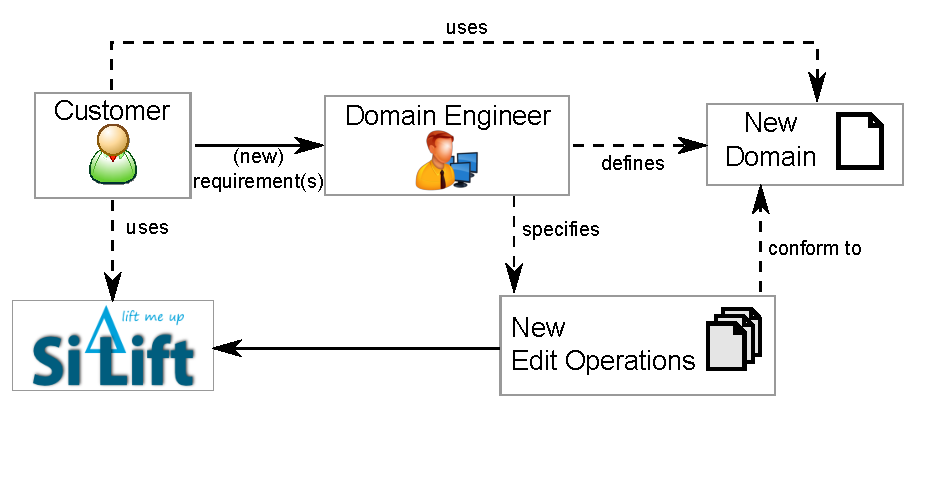
\includegraphics[width=0.9\textwidth]{images/overview}
  \end{center}
\end{frame}
\begin{frame}
\frametitle{New Domain - New Pain}
\begin{center}
\includegraphics[scale=0.8]{images/motivation}
  \end{center}
\end{frame}
\begin{frame}
\frametitle{New Domain - Less Pain}
Support the Domain Engineer:
\begin{itemize}
  \item Offer a framework for defining and using edit operations (see [1])
\item Tight Eclipse Integration(Wizards, Dialogues, Views, \ldots)
\item Generate a \textbf{basic} set of edit operations \textbf{automatically} (see [2])
\item \textbf{Validate} edit operations according to tool mechanisms
\item Build derived artifacts \textbf{automatically}
\item Offer automatic \textbf{Quickfix} if available
\end{itemize}
\bigskip
{\footnotesize{
\textbf{[1]}T. Kehrer, U. Kelter, and G. Taentzer, ``Consistency-preserving edit scripts in model
versioning'',in ASE 2013\\
\medskip
\textbf{[2]}M. Rindt, T. Kehrer, U. Kelter, ``Automatic Generation of Consistency-Preserving Edit
Operations for MDE Tools'',in Models 2014}}
\end{frame}